\subsubsection{Bends} 

Flow in curved pipes may be significantly impeded due to the effects of surface friction, secondary flow and flow separation. The resistance in a pipe bend may be modelled in a similar way to a valve but with the loss coefficient modified to account for the bend geometry and flow conditions. For a bend in a pipe $j$ of diameter $d_j$, bend angle $0 < \alpha_j < \pi$ and bend radius $r_j$, as shown in figure \ref{fig:bend_diagram}, the resistance may be defined by as
\begin{align}\label{bend_resistance}
\boxed{
  \!\begin{gathered}
  R_j = - \frac{k_j Q_j|Q_j| }{2 A_j} + g A_j \Delta H_j \hspace{0.5cm} \text{where}\\
  k_j = f_j \alpha_j \frac{r_j}{d_j}	 + (0.1 + 2.4 f_j) \sin \left( \frac{\alpha_j}{2} \right) + \frac{6.6 f_j \left[ \sqrt{\sin \left( \frac{\alpha_j}{2} \right) } + \sin \left( \frac{\alpha_j}{2} \right)  \right] }{\left(\frac{r_j}{d_j} \right)^{\frac{4 \alpha_j}{\pi}}}.
  \end{gathered}
}
\end{align}
Here $f_j = f(Q_j)$ is the friction factor which may also be a function of the pipe roughness. This empirical equation, see \cite{rennels22}, is one of a number of possible methods for determining loss coefficients for pipe bends; different methods may be preferred in certain situations. For equation \eqref{bend_resistance} to be valid it is required that $r_j / d_j \geq 0.5$.


\begin{figure}
\centering
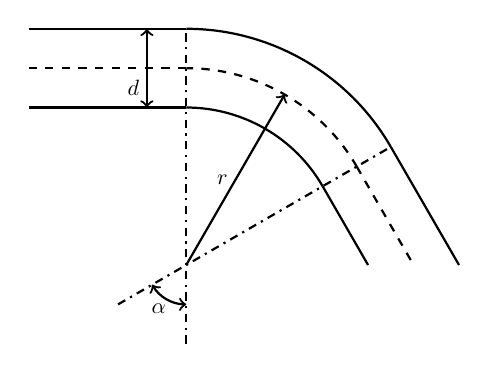
\begin{tikzpicture}[ scale=1, every node/.style={scale=0.8},] 
\draw[thick, dash dot] (0,-1) -- (0,3);
\draw[thick, dash dot] (-0.866,-0.5) -- (2.598,1.5);
% Inlet pipe
\draw[thick] (0,2) -- (-2,2);
\draw[thick, dashed] (0,2.5) -- (-2,2.5);
\draw[thick] (0,3) -- (-2,3);
% Bend
\draw[thick] (1.732,1) arc (30:90:2);
\draw[thick, dashed] (2.165,1.25) arc (30:90:2.5);
\draw[thick] (2.598,1.5) arc (30:90:3);
% Outlet pipe
\draw[thick] (1.732,1) -- (2.309,0);
\draw[thick, dashed] (2.165,1.25) -- (2.887,0);
\draw[thick] (2.598,1.5) -- (3.464,0);
% Annotations
\node[anchor=east] at (-0.5,2.25) {$d$};
\draw[thick, <->] (-0.5,2) -- (-0.5,3);
\draw[thick, <->] (-0.433,-0.25) arc (30:90:-0.5);
\node[anchor=north] at (-0.35,-0.39) {$\alpha$};
\draw[thick, ->] (0,0) -- (1.25,2.165);
\node[anchor=east] at (0.625,1.082) {$r$};
\end{tikzpicture} 
\caption{A bend in a pipe of diameter $d$ with a bend radius $r$ and bend angle $\alpha$.}
\label{fig:bend_diagram}
\end{figure}